\documentclass[../thesis.tex]{subfiles}
% Separate preamble for this subfile. This preamble is loaded last, so one can override various functions before \begin{document}

% Better comment extension for Vscode colors these comments differently
% Normal comment color
% * Important information
% ! ALERT
% ? Question
% TODO stuff to do
% // This is strikethrough


\begin{document}

\mycomment{

Den tiden som gjennstår:


Jo høyere dimensjon vi får jo mer eksotisk kan disse tilingene bli. Står noe referanser til i paperet. 
Keller hadde en teori om at enhver tiling må være av den typen -- (Se for deg enhetskuben i 2D)
enhver tiling nødvendigvis medføre at,
alle tiles har en full felles kant med en annen tile

i 2D gjelder det her med at man har to kanter hvor man har en full felles kant (med den over og den under)


i 1D har man ingen sidekant, det er et punkt
men poenget er at i veldig høye dimensjoner så kan tilingene bli mer eksotiske, og et utrykk for det er at du ikke trenger å ha en full kant med noen som helst annen tile
dimensjon > 7


%! 
-> når det er større en 1 har vi flere muligheter

-> en begrensing legges av Kellers theorem, 
}

Informally, to tile refers to the process of covering some surface with objects. These objects are called tiles and come in a variety of shapes and sizes. When we are tiling, we essentially place copies of the tile next to each other in a systematic way, intending to leave no gaps and no overlaps between the tiles. The resulting tiling can be as simple as the one shown in \cref{fig:tiling_one} where we have used a single tile, the unit square, to tile the plane, or as complex as \cref{fig:tiling_two} where we have used four different tiles to tile the plane. The first is an example of what is known as a \emph{monohedral tiling} in which all tiles are congruent \cite[p. 20]{grunbaumTilingsPatterns1987}, and the latter is an example of a Penrose tiling which are well known for being non-periodic \cite{penrosePentaplexityClassNonPeriodic1979}. %* 1979 page 535 har også penrose tilings
% non-periodic tiling, meaning that there is no period parallelogram \SigridChange{KORT FORTALT}.  % Worth emphasizing is the fact that we lack a method for determining whether a tile is the prototile of a monohedral tiling 




\begin{figure}[h!]%h!
    \centering
    \begin{subfigure}{.47\textwidth}
        \centering
        %\includegraphics[width=0.9\linewidth]{spec_no_shift.jpg}
        %* Figure 1
        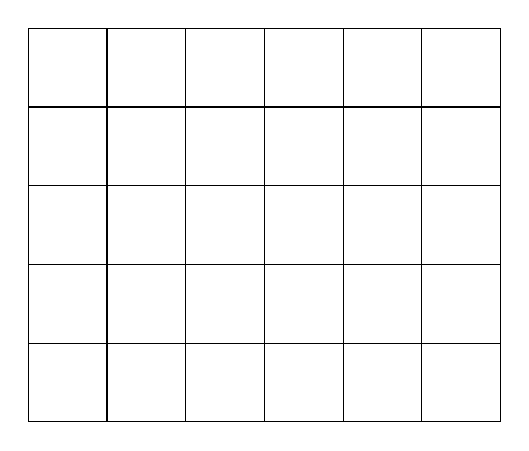
\begin{tikzpicture}[scale=1]
            % Define the tile
            \def\tile{
              % Draw the unit square
              \draw (0,0) rectangle (1,1);
            }
          
            % Draw the tiling pattern
            \foreach \x in {0,1,2,3,4,5}{
              \foreach \y in {0,1,2,3,4}{
                \pgfmathsetmacro{\shiftX}{\x} % Set horizontal shift
                \pgfmathsetmacro{\shiftY}{\y} % Set vertical shift
                \begin{scope}[shift={(\shiftX,\shiftY)}]
                  \tile % Draw the tile
                \end{scope}
              }
            }
        \end{tikzpicture}
        %* —————————————————
        \caption{Lattice spectra}
        \label{fig:tiling_one}
    \end{subfigure}\quad
    \begin{subfigure}{.47\textwidth}
        \centering
        \includegraphics[width=0.9\linewidth]{Penrose_Tiling_.png}
        \caption{P1 Penrose Tiling}
        \label{fig:tiling_two}
    \end{subfigure}
    \caption{Penrose original aperiodic tiling \cite{penrosePentaplexityClassNonPeriodic1979}, from \cite{inductiveloadP1TilingUsing}, forklare fargelegginen, \SigridComment{By Inductiveload - Own work, Public Domain, https://commons.wikimedia.org/w/index.php?curid=5839133}}
    \label{fig:tilingsss}
\end{figure}


Another interesting monohedral tiling is given in \cref{fig:tiling_three}. This is an example of an Escher tiling in which a lizard tiles the plane \cite{kolountzakisTilingsTranslation2010}. Note that in comparison to the square tilings in \cref{fig:tiling_one}, there is important to highlight a fundamental difference between the square and lizard tilings. In the latter, one needs to rotate the lizard tile in order to cover the entire surface. 
Last, in addition to translation and rotation, one can have reflections \cite{grunbaumTilingsPatterns1987}. Although this is not exactly shown in any figure, one can find reflection points/lines for parts of the tiles in \cref{fig:tilings_one_two,fig:tiling_three}. 
\SigridComment{how does this work for the lattice tile? Does one consider it to have an infinite amount of reflection lines or none at all?}
% However, it is essential to highlight a fundamental difference between the square tilings in \cref{fig:tiling_one} and the lizard tilings in \cref{fig:tiling_three}. In the latter, one needs to rotate the tile in order to cover the entire surface. 

\mycomment{ %! If we bring in reflection —— We don't ——
However, it is important to highlight a fundamental difference between the square tilings in \cref{fig:tiling_one}, the lizard tilings in \cref{fig:tiling_three}, and the BLABLA tilings in \cref{fig:tiling_four}. Each represents a way to cover the entire surface exclusively using either translation, rotation, or reflection in that order.  
% OPTION 1: Delete "in that order" and write: Meaning square tilings need only translation to cover the entire surface, lizard tilings need only rotation, and BLABLA only needs reflection.
% OPTION2: It means square tilings can cover the entire surface using translation, lizard tilings need only rotation, and BLABLA only needs reflection. 
% OPTION 3: The first, \cref{fig:tiling_one}, can tile the surface using translation only, \cref{fig:tiling_three} can tile using rotation only, and \cref{fig:tiling_four} can tile using reflection only.
}
%  https://www.wikiart.org/en/m-c-escher/flying-fish    
%  https://www.wikiart.org/en/m-c-escher/lizard-1} 

\begin{figure}[t]%h!
    \centering
    \includegraphics[width=0.4\linewidth]{lizard-1.jpg}
    \caption{Lizard from \cite{m.c.escherLizard1942}}
    \label{fig:tiling_three}
\end{figure}


\mycomment{  %! Block comment
\begin{figure}[t]%h!
    \centering
    \begin{subfigure}{.47\textwidth}
        \centering
        \includegraphics[width=0.9\linewidth]{lizard-1.jpg}
        \caption{Lizard}
        %\label{fig:tiling_three}
    \end{subfigure}\quad
    \begin{subfigure}{.47\textwidth}
        \centering
        \includegraphics[width=0.9\linewidth]{flying-fish.jpg}
        \caption{Flying fish}
        \label{fig:tiling_four}
    \end{subfigure}
    \caption{from \cite{m.c.escherLizard1942}}
    \label{fig:tilingsss_two}
\end{figure}
}

However interesting the Penrose and Escher tilings appear, we will only focus on tilings of $\R^d$ by translation and using only the unit cube as our tile. Considering only cube-tilings might seem simple initially, but we will see that as we increase the dimension, we get increased flexibility and more complex tilings. It turns out that in higher dimensions, highly exotic and counterintuitive cube tilings exist. The fact that this kind of tiling exists in the first place is surprising in light of Keller's theorem \cite{iosevichSpectralTilingProperties1998}.  %This is Perhaps surprising in light of Keller's theorem. 

%\begin{theorem}  %* (My original) Keller theorem from the paper of Iosovich and Pedersen
%    Given a discrete subset $T\subset \R^d$. If $T$ is a tiling set for $\Omega$, then given any pair $\lambda, \lambda' \in T$ such that $\lambda\neq\lambda'$, there exists a $j\in \braq{1,\dots,d}$ so that $\bral{t_j -t_j' } \in \N$
%\end{theorem}
%\begin{theorem}  %* Keller theorem from the paper of Lagarias and Reeds
%    If $\Lambda + \bras{0,1}^n$ is a tiling of $\R^n$, then each $\lambda,\lambda'\in \Lambda$ has
%    \begin{equation*}
%        \lambda_i - \lambda_i' \in \intnozero \quad \text{ for some } i, \quad 1\leq i \leq n.
%    \end{equation*}
%\end{theorem}
\begin{theorem}[Keller's Theorem]\label{thrm:keller_tiling}
    Let $\Lambda \subset \R^d$ be a discrete subset. If $\Lambda$ is a tiling set for the unit cube $\bras{0,1}^d$, then given any pair $\lambda, \lambda' \in \Lambda$ such that $\lambda\neq\lambda'$, there exists a $j\in \braq{1,\dots,d}$ so that $\lambda_j -\lambda_j' \in \intnozero$.
\end{theorem}
%? ——————————————————————————————————  Info  ——————————————————————————————————
%? Timeline. Keller's theorem and conjecture are both from Keller's paper from 1930. Although, they are never stated as "Keller's theorem"  or "Keller's Conjecture" until after. At least, that is my Thought. I think the first time these names appears is in a paper by his student Perron in 1940.
%? ——————————————————————————————————  Short version [Kellers Theorem]  ——————————————————————————————————
%? Kellers theorem was prooved by Keller \cite{ott-heinrichkellerUberLuckenloseErfullung1930} in 1930. A detailed proof appears in Perron \cite{perronUeberLueckenloseAusfuellung1940} satz 9 in chapter 3 on page 11. Source for this is \cite[p. 8]{iosevichSpectralTilingProperties1998}. Furthermore, Perron writes in the intro of his paper \cite{perronUeberLueckenloseAusfuellung1940} that Keller proved his theorem and will do this in chapter 3 while adding some more info to the problem (blue). Additionally, it is important to mention that in Remark 1.2 in \cite{iosevichSpectralTilingProperties1998}, they present Theorem 1.1, which is essentially my master, and some valuable insight into the importance of this, as well as on the topic of exotic tilings.
%? ——————————————————————————————————  Short version [Kellers Conjecture]  ——————————————————————————————————
%? In their paper \cite[p. 2]{iosevichSpectralTilingProperties1998}, they briefly introduce the problem's history. They state, "Keller, while working on Minkowski's conjecture, made the stronger conjecture that one could omit the lattice assumption in Minkowski's conjecture." Furthermore, Perron, in the intro of his paper \cite{perronUeberLueckenloseAusfuellung1940}, discusses this further. The most interesting part is that Keller later doubted his conjecture. He also states that Keller only sketched the proof and that it was hard to follow for dimensions 5 and 6. Worth mentioning that Perron proves this for $n \leq 6$. Furthermore, The paper on the resolution of Keller's conjecture \cite{brakensiekResolutionKellerConjecture2020} states that the conjecture originates from \cite{kellerUberLuckenloseErfullung1930}. They also write that Perron proved this over two papers (the one above and in a paper I have downloaded but not cited) and that Minkowski's conjecture was proved in 1942 by Hajós (no citation here).
%? ——————————————————————————————————  Sigrid Note  ——————————————————————————————————
%? The existence of exotic tilings is perhaps surprising in light of Keller's theorem. If anything, Sigrid would say that the conjecture hints at the opposite. That such exotic tilings do NOT exist. That is to say, Keller made the thoughts that led to his conjecture after he had proved his theorem (or while doing it). He also later doubted this (see intro in Perron). Sigrid emphasizes that if one can show the integer difference independent of the lattice assumption (and dimension), then it is reasonable to assume that one can strengthen the Minkowski conjecture into Keller's conjecture. By lattice assumption, we mean that the integer difference exists whether it is a lattice or not. It is important to remark that the conjecture does not support that exotic tilings should exist. Rather, the opposite. It indicates some rigidity. However, as we know it to be untrue for $d>7$, we have that these exotic tilings appear. 

%* Hvis jeg kan vise at jeg alltid har denne heltalls-differansen så er det naturlig å anta at jeg kan styrke denne mikovsky conjecturen.
%* Dette er fordi  han viser theoremet uavhengig av om det er en lattice eller ikke

%* Derfor blir følgende er ikke helt riktig:
%* "One indicator of this characteristic follows from Keller's conjecture \cite{ott-heinrichkellerUberLuckenloseErfullung1930}."

\SigridComment{Difficult transition here }

Although Keller proved the theorem in his original paper \cite{kellerUberLuckenloseErfullung1930}, Iosevich and Pedersen also provide an English proof in their paper \cite{iosevichSpectralTilingProperties1998}. Furthermore, in the same paper by Keller, he also conjectured the following. \SigridChange{/} Additionally, the same paper by Keller also conjectured the following. \SigridChange{/} Following his theorem, Keller also conjectured the following. %In the same paper, Keller conjectured the following. % Keller conjectured that

\begin{conjecture}[Keller's conjecture]
    All tilings of $\R^d$ by translations of the unit cube contain two cubes that share an entire $(d-1)$-dimensional face.
\end{conjecture}

%* Known to be true... d<=7, but in fact false when d>7...
%* For å kaste lys på at de kan være eksotiske så er det det at de er usant over 7 som er det relevante her. 
If the dimension is two, the squares share an edge; if the dimension is three, they share a face. It is important to remark/emphasize that the conjecture does not support the existence of exotic tilings. Instead, it indicates the opposite — rigidity in the tiling of the space/$\R^d$. However, after it was recently proven true in dimension seven, we now know the conjecture to be false for all $d>7$ \cite{brakensiekResolutionKellerConjecture2020}. 

\SigridComment{same, but opposite order of the second statement. I have a preference for the first, but it might be wrong in terms of the use of "however" here.}

If the dimension is two, the squares share an edge; if the dimension is three, they share a face. It is important to remark/emphasize that the conjecture indicates a rigidity in the tiling of the space/$\R^d$. It does not indicate the existence of exotic tilings. However, after it was recently proven true in dimension seven, we now know the conjecture to be false for all $d>7$ \cite{brakensiekResolutionKellerConjecture2020}.


It is precisely in the higher dimensions where Keller's conjecture fails that we get the tilings we consider highly exotic and counterintuitive.

\SigridComment{Other, variants. not quite sure what terminology to use}

It is \SigridChange{these} higher dimensional tilings we \SigridChange{consider to be/categorize as /classify as} highly exotic and counterintuitive.\\
/ It is precisely where Keller's conjecture fails that we get the tilings \SigridChange{that are both/we consider to be/categorize/classify as} highly exotic and counterintuitive. %both


\SigridChange{ ———————————}


% This conjecture does not support the fact that exotic tilings could exist, as it indicates a rigidity in tiling the space. However, it is now known to be false for all dimensions greater than seven after being proven true in dimension seven.

% It is the higher dimensional tilings in which two cubes do not share an entire $(d-1)$-dimensional face we classify as being exotic and counterintuitive.
% It is these higher dimensional tilings in which the property of two cubes not sharing an entire $(d-1)$-dimensional face that makes so the tilings are considered highly exotic and counterintuitive. 
% These higher dimensional tilings in which the property of two cubes not sharing an entire $(d-1)$-dimensional face make the tilings highly exotic and counterintuitive. 
%  as we now know the conjecture to be false for all dimensions greater than seven, we have that these exotic tilings do exist. 
%* ———————————————————————————— Tilings ——————————————————
%* Tenk overgang, vurder intro med non overlappings og coverings, litt uformelt, ingen def, dvs det fra gammelt med gammel struktur og så lede over til vår def
% In defining tilings formally, we use indicator functions \cite{kolountzakisTilingsTranslation2010}. 
\SigridComment{Sigrid laid out two options here. I have tried incorporating the second option by defining it with "words" and a bit more informally so that I only have \emph{one} formal definition of tilings.}
In defining tilings more formally/rigorously/using our geometric intuition/$\dots$, one often defines it as a non-overlapping covering of the space \cite{iosevichSpectralTilingProperties1998}. By this, we mean that a subset $\Omega \subset \R^d$ of non-zero measure is a tile, and a set $\Lambda \subset \R^d$ is a tiling set if they satisfy both of the following conditions. First, (the union of) $\Omega+\lambda$ for (all) $\lambda \in \Lambda$ must cover $\R^d$ up to measure zero. Secondly, all intersections $(\Omega+\lambda) \cap (\Omega+\lambda')$ of distinct elements $\lambda,\lambda' \in \Lambda$ must have measure zero. Note that $\Omega+\lambda$ denotes the translate of $\Omega$ by the vector $\lambda$. More formally/Nevertheless, tilings can also be expressed using indicator functions as follows \cite{kolountzakisTilingsTranslation2010}. \SigridChange{/} We will, however, define tilings in terms of indicator functions as follows \cite{kolountzakisTilingsTranslation2010}.
% Rather than defining tiling in terms of a non-overlapping covering of the space, we will instead define tiling by the indicator function, using little of our geometric intuition \cite{kolountzakisTilingsTranslation2010} \cite{kolountzakisStudyTranslationalTiling2003}. 
\begin{definition}[Tiling set]\label{def:tiling}
    Let $\Omega \subset \R^d$ be a subset with nonzero measure, and consider a \SigridChange{discrete (or just a set?)} set $\Lambda \subset \R^d$. If
    \begin{equation}\label{eq:tiling_set}
        \sum_{\lambda \in \Lambda} \indicator{\Omega}{x-\lambda} = 1, \text{\space} a.e. \quad x \in \R^d,
    \end{equation}
    then $\Omega$ is called a \emph{tile}, and $\Lambda$ is called a \emph{tiling set} for $\Omega$. We say that $(\Omega, \Lambda)$ is a \emph{tiling pair}.
\end{definition}
\begin{remark}
    We can also say that $\Omega$ \emph{tiles $\R^d$ by translation}, or that $\Omega$ is a \emph{tiling} of $\R^d$. 
\end{remark}
\begin{remark}
    One can define tilings more generally. By this, we mean that in place of the indicator function, we can have a non-negative, integrable function $f$. Other than allowing for any other constant value than $1$, the definition is the same. \textcolor{orange}{Note that we still require the same constant value almost everywhere.} The reader is referred to \cite{kolountzakisTilingsTranslation2010} for more details on this topic. \SigridComment{1. Is the last sentence worth mentioning? 2. is the orange sentence an unnecessary note, as there is little ambiguity in the previous sentence? 3. is this whole remark unnecessary? That is, it is better to leave it out and move on. Am I diving too much into tilings in general and moving away from the "red thread" of the link between spectra and tilings.}
\end{remark}

\SigridComment{remarks, or direct in text}


In other words, we can also say that $\Omega$ \emph{tiles $\R^d$ by translation}, or that $\Omega$ is a \emph{tiling} of $\R^d$. Additionally, one can define tilings more generally. By this, we mean that in place of the indicator function, we can have a non-negative, integrable function $f$. Other than allowing for any other constant value than $1$, the definition is the same. Note that we still require the same constant value almost everywhere. The reader is referred to \cite{kolountzakisTilingsTranslation2010} for more details on this topic.
%* ———————————————————————————— One dimension  ——————————————————
%* Viktig, må inn en bit her om 
%* som en konsekvens av Kellers theorem så får vi nå akkurat den samme formen på disse tilings settene 
%* de må ligge inneholt i akkurat de samme typene mengder, og de kan ikke være ekte mindre for da får vi ikke oppfylt tiling kravet mitt.
\SigridChange{(continue here)} If we now restrict our attention to the unit cube in d-dimensions, Keller's theorem immediately gives the following for $d=1$. Here, the unit cube is simply the unit interval $I = \bras{0,1}$. %In dimension one, the unit cube is simply the unit interval $I = \bras{0,1}$. 

\begin{lemma}\label{lem:tiling_unit_1d}
    The set $\Lambda = \Z +\alpha$ for some value $\alpha\in \R$ constitutes a tiling set for $I$.
\end{lemma}
%\begin{theorem}  %* Bruker alle elementene i T for å flytte på I, da dekker vi hele $\R$.  
%    Let $\Omega = I$. If $T=\Z$, then $T$ is a tiling set for $I$.
%\end{theorem}

\begin{proof}  % This follows directly from \cref{thrm:keller_tiling}. Take $\lambda, \lambda' \in \Lambda$. 
    %  Må konkret gå tilbake til definisjonen du har valgt. For den kan vi bruke eksplisitt til å si:
    %Det Keller's theorem forteller meg, er at jeg må ha noe som er en undermengde av $\Lambda = \Z + \alpha$, og i og med at jeg må ha 1 almost everywhere, så gjør det at hvis jeg tar bort et punkt fra $\Lambda$ slik at vi har $\Lambda \subset \Z + \alpha$, så vil jeg få et intervall hvor jeg har 0.
    %  La oss nå si at et punkt er utelatt. Det betyr at $\sum \indicator{\Omega}{t} = 0$ og vi kan si nøyaktig hvor det er null, for det er på det punktet vi har utelatt. Dvs, $x\in I+\lambda'$, hvor $\lambda'$ er punktet vi utelot fra flisleggingsmengden. Videre, så er målet av $I+\lambda'$ positivt, det er ikke neglisjerbart. Dvs, der du ikke har verdien 1, de områdene, de er ikke neglisjerbare. Og videre vet vi at vi har $x\in I+\lambda'$, dvs et helt slikt interval, hvor $\sum \indicator{\Omega}{t} = 0$, og dette området har positivt mål. 
    Let $\Lambda \subset \R^d$. Using \cref{thrm:keller_tiling}, we instantly get that there must be an integer distance between two distinct points $\lambda,\lambda' \in \Lambda$ in a tiling set for $I$ \SigridChange{/} if $\Lambda$ is to be a tiling set for $I$. Hence, we know that $\Lambda \subseteq \Z +\alpha$. Now, given an arbitrary point $\lambda' \in \Z +\alpha$, assume that $\lambda'\notin \Lambda$ so that we have a case where $\Lambda \subset \Z+\alpha$. However, by using \cref{def:tiling}, observe now that we have an entire interval, specifically $I+\lambda'$, where $\indicator{I}{x - \lambda'} = 0$. As $\mes{I+\lambda'} = 1 $, we do not have
    \begin{equation*}
        \sum_{\lambda \in \Lambda\setminus \braq{\lambda'}} \indicator{I}{x-\lambda} = 1, \text{\space} a.e. \quad x \in \R^d.
    \end{equation*}
    That is, we have a non-negligible region with a value not equal to one. Hence $\lambda' \in \Lambda$, which shows that $\Lambda = \Z+\alpha$ and that $\Lambda$ is a tiling set for $I$. %for a tiling set $\Lambda$ of $I$.
\end{proof}

Increasing the dimension by one,


\SigridComment{to be continued...}
%* Mention here in the figure of 2D the link with Keller's conjecture. Two squares share a face. 


%* change the lattice tiling 



\begin{figure}[t]%h!
    \centering
    \begin{subfigure}{.47\textwidth}
        \centering
        %\includegraphics[width=0.9\linewidth]{spec_no_shift.jpg}
        %* Figure 1
        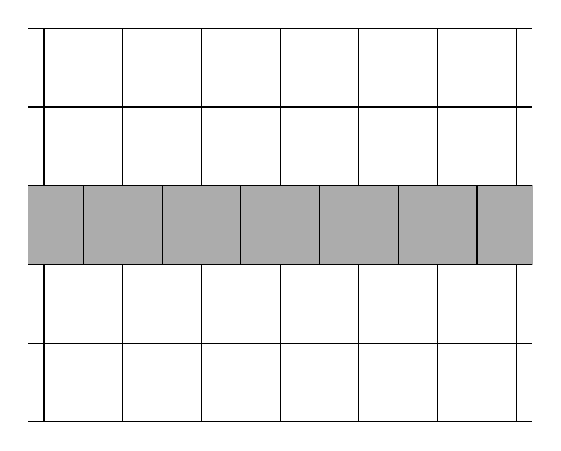
\begin{tikzpicture}[scale=1]
            % Define the tile
            \def\tile{
            \draw[fill=white] (0,0) rectangle (1,1);
            }
            \def\tiletwo{
            \draw[fill=gray!65] (0,0) rectangle (1,1);
            }
            
            % Draw the tiling pattern
            % Everything else
            \foreach \y in {0,1,3,4}{
                \foreach \x in {0,1,2,3,4,5}{
                    \pgfmathsetmacro{\shiftX}{\x} % Set horizontal shift
                    \pgfmathsetmacro{\shiftY}{\y}
                    \begin{scope}[shift={(\shiftX,\shiftY)}]
                        \tile
                    \end{scope}
                }
            }
            % Shifted line
            \foreach \x in {0}{
            \draw[gray!65, fill=gray!65] (\x-0.2,2) rectangle (\x+0.5,3);
            }
            \foreach \x in {6}{
            \draw[gray!65, fill=gray!65] (\x+0.2,2) rectangle (\x-0.5,3);
            }
            % Middle line, must be after the above code in order to get black lines at correct spots
            \foreach \y in {2}{
                \foreach \x in {0,1,2,3,4}{
                    \pgfmathsetmacro{\shiftX}{\x+0.5} % Set horizontal shift
                    \pgfmathsetmacro{\shiftY}{\y}
                    \begin{scope}[shift={(\shiftX,\shiftY)}]
                        \tiletwo
                    \end{scope}
                }
            }
            % small black lines at the top and bottom
            \foreach \y in {0,1,2,3,4,5}{
                \draw (0-0.2,\y) -- (6+0.2,\y);
            }
        \end{tikzpicture}
        %* —————————————————
        \caption{Single row shift}
        \label{fig:single_shift_horizontal_tiling}
    \end{subfigure}\quad
    \begin{subfigure}{.47\textwidth}
        \centering
        %\includegraphics[width=0.9\linewidth]{spec_single_shift.jpg}
        %* Figure 2
        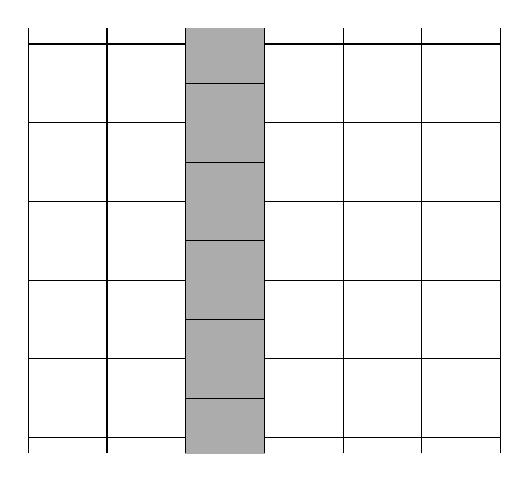
\begin{tikzpicture}[scale=1]
            % Define the tile
            \def\tile{
            \draw[fill=white] (0,0) rectangle (1,1);
            }
            \def\tiletwo{
            \draw[fill=gray!65] (0,0) rectangle (1,1);
            }
            
            % Draw the tiling pattern
            % Everything else
            \foreach \x in {0,1,3,4,5}{
                \foreach \y in {0,1,2,3,4}{
                    \pgfmathsetmacro{\shiftX}{\x} % Set horizontal shift
                    \pgfmathsetmacro{\shiftY}{\y}
                    \begin{scope}[shift={(\shiftX,\shiftY)}]
                        \tile
                    \end{scope}
                }
            }
            % Shifted line
            \foreach \y in {0}{
            \draw[gray!65, fill=gray!65] (2,\y-0.2) rectangle (3,\y+0.5);
            }
            \foreach \y in {5}{
            \draw[gray!65, fill=gray!65] (2,\y+0.2) rectangle (3,\y-0.5);
            }
            % Middle line, must be after the above code in order to get black lines at correct spots
            \foreach \x in {2}{
                \foreach \y in {0,1,2,3}{
                    \pgfmathsetmacro{\shiftX}{\x} % Set horizontal shift
                    \pgfmathsetmacro{\shiftY}{\y+0.5}
                    \begin{scope}[shift={(\shiftX,\shiftY)}]
                        \tiletwo
                    \end{scope}
                }
            }
            % small black lines at the top and bottom
            \foreach \x in {0,1,2,3,4,5,6}{
                \draw (\x,0-0.2) -- (\x,5+0.2);
            }
        \end{tikzpicture}
        %* —————————————————
        \caption{Single column shift}
        \label{fig:single_shift_vertical_tiling}
    \end{subfigure}\\
    \begin{subfigure}{.47\textwidth}
        \centering
        %\includegraphics[width=0.9\linewidth]{multiple_shift_left_zero.jpg}
        %* Figure 3
        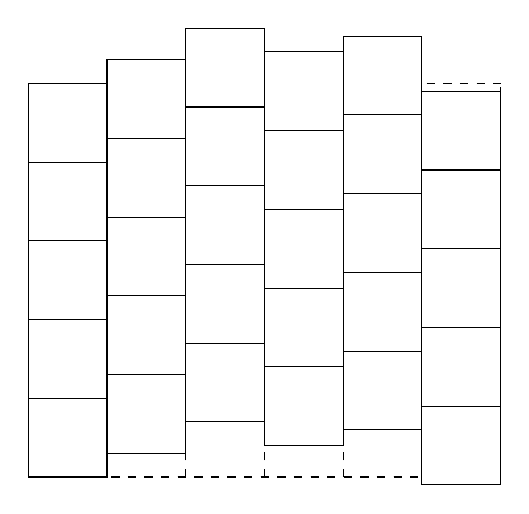
\begin{tikzpicture}[scale=1]
            % Define the tile
            \def\tile{
            % Draw the unit square
            \draw[fill=white] (0,0) rectangle (1,1);
            }

            % Shift list
            \def\BetaMinOne{0}
            \def\BetaZero{0.3}
            \def\BetaOne{0.7}
            \def\BetaTwo{0.4}
            \def\BetaThree{0.6}
            \def\BetaFour{-0.1}
            
            

% Axis lines
%\draw[->] (-1.5,0) -- (4.5,0) node[right] {$X$};
%\draw[->] (0,-1.5) -- (0,3.5) node[above] {$Y$};
\draw[dashed] (0,0) -- (6,0);
\draw[dashed] (0,0) -- (0,5);

% Dashed lines at each integer in the x direction
\foreach \x in {0,...,6}
    \draw[dashed] (\x,0) -- (\x,5);

% Dashed lines at each integer in the y direction
\foreach \y in {0,...,5}
    \draw[dashed] (0,\y) -- (6,\y);


            % Draw the tiling pattern
            \foreach \x in {0,1,2,3,4,5}{
            \foreach \y in {0,1,2,3,4}{
                \ifnum\x=0 % Set vertical shift for the third column only
                    \pgfmathsetmacro{\shiftX}{\x} % No vertical shift for other columns
                    \pgfmathsetmacro{\shiftY}{\y + \BetaMinOne} % Shift one unit upward
                \fi
                \ifnum\x=1
                    \pgfmathsetmacro{\shiftX}{\x}
                    \pgfmathsetmacro{\shiftY}{\y + \BetaZero}
                \fi
                \ifnum\x=2
                    \pgfmathsetmacro{\shiftX}{\x} 
                    \pgfmathsetmacro{\shiftY}{\y + \BetaOne} 
                \fi
                \ifnum\x=3
                    \pgfmathsetmacro{\shiftX}{\x}
                    \pgfmathsetmacro{\shiftY}{\y + \BetaTwo}
                \fi
                \ifnum\x=4
                    \pgfmathsetmacro{\shiftX}{\x}
                    \pgfmathsetmacro{\shiftY}{\y + \BetaThree}
                \fi
                \ifnum\x=5
                    \pgfmathsetmacro{\shiftX}{\x}
                    \pgfmathsetmacro{\shiftY}{\y + \BetaFour}
                \fi
                \begin{scope}[shift={(\shiftX,\shiftY)}]
                \tile % Draw the tile
                \end{scope}
            }}
        \end{tikzpicture}
        %* —————————————————
        \caption{Multiple shifts vertical}
        \label{fig:multiple_shift_vertical_tiling}
    \end{subfigure}\quad
    \begin{subfigure}{.47\textwidth}
        \centering
        %\includegraphics[width=0.9\linewidth]{multiple_shift_left_zero_horizontal.jpg}
        %* Figure 4
        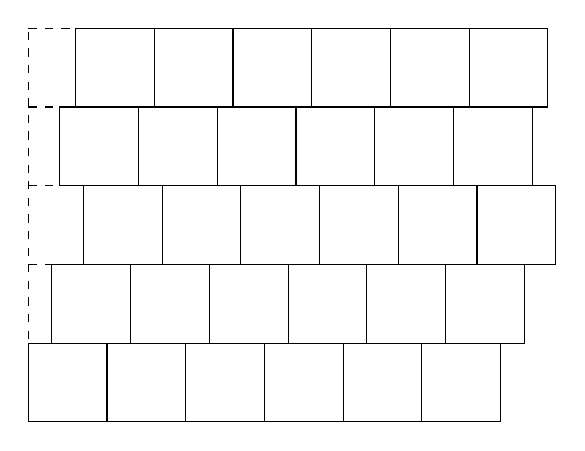
\begin{tikzpicture}[scale=1]
            % Define the tile
            \def\tile{
            % Draw the unit square
            \draw[fill=white] (0,0) rectangle (1,1);
            }

            % Shift list
            \def\BetaMinOne{0}
            \def\BetaZero{0.3}
            \def\BetaOne{0.7}
            \def\BetaTwo{0.4}
            \def\BetaThree{0.6}
            
            

% Axis lines
%\draw[->] (-1.5,0) -- (4.5,0) node[right] {$X$};
%\draw[->] (0,-1.5) -- (0,3.5) node[above] {$Y$};
\draw[dashed] (0,0) -- (6,0);
\draw[dashed] (0,0) -- (0,5);

% Dashed lines at each integer in the x direction
\foreach \x in {0,...,6}
    \draw[dashed] (\x,0) -- (\x,5);

% Dashed lines at each integer in the y direction
\foreach \y in {0,...,5}
    \draw[dashed] (0,\y) -- (6,\y);


            % Draw the tiling pattern
            \foreach \x in {0,1,2,3,4,5}{
            \foreach \y in {0,1,2,3,4}{
                \ifnum\y=0
                    \pgfmathsetmacro{\shiftX}{\x + \BetaMinOne}
                    \pgfmathsetmacro{\shiftY}{\y}
                \fi
                \ifnum\y=1
                    \pgfmathsetmacro{\shiftX}{\x + \BetaZero}
                    \pgfmathsetmacro{\shiftY}{\y}
                \fi
                \ifnum\y=2
                    \pgfmathsetmacro{\shiftX}{\x + \BetaOne} 
                    \pgfmathsetmacro{\shiftY}{\y} 
                \fi
                \ifnum\y=3
                    \pgfmathsetmacro{\shiftX}{\x + \BetaTwo}
                    \pgfmathsetmacro{\shiftY}{\y}
                \fi
                \ifnum\y=4
                    \pgfmathsetmacro{\shiftX}{\x + \BetaThree}
                    \pgfmathsetmacro{\shiftY}{\y}
                \fi
                \begin{scope}[shift={(\shiftX,\shiftY)}]
                \tile % Draw the tile
                \end{scope}
            }}
        \end{tikzpicture}
        %* —————————————————
        \caption{Multiple shifts horizontal}
        \label{fig:multiple_shift_horizontal_tiling}
    \end{subfigure}
    \caption{Text}
    \label{fig:tiling_figures}
\end{figure}

\end{document}


